% =========================================================================
% Validation chapter section: the Japanese field-case campaign.
% Drop-in for the validation chapter (placement note: written as a chapter
% section rather than an appendix because it carries interpretive findings
% that condition how the Phase 1 results should be read; the per-case
% audit records remain in the repository under docs/validation/).
%
% New BibLaTeX keys required (entries to add to the thesis .bib):
%   okamura_gounokawa_2025   Okamura et al. (2025), Soils Found. 65:101656
%   sako_gounokawa_2019      Sako et al. (2019), JSCE J. B1 75(1):279-290
%   yabe_levee_committee_2013   Yabe River Levee Investigation Committee (2013)
%   tokoro_levee_committee_2017 Tokoro River Levee Investigation Committee (2017)
%   waseda_gounokawa_dataset_2025  companion dataset doi:10.20556/0002006234
% Existing keys reused: sellmeijer_2011, pol_sie_2024, pol_compgeo_2024,
%   pol_thesis_2022, van_beek_2015, terzaghi1943, schweckendiek_2014.
% Figure paths assume the two campaign figures are copied into the thesis
% figures directory; adjust \includegraphics paths as needed.
% =========================================================================

\section{Validation Against Japanese Field Cases}
\label{sec: Validation Against Japanese Field Cases}

The physics kernels of the Phase~1 engine were verified against their source
experiments: the critical-head model against the IJkdijk fine-tuning cases of
\textcite{sellmeijer_2011}, and the progression rate law against the
small-scale and large-scale time-dependent experiments underlying
\textcite{pol_compgeo_2024}. Those references are, however, Dutch sand cases
at low gradients, whereas the Tokachi and Satsunai study levees stand on
coarse, highly transmissive foundations loaded by flashy typhoon hydrographs.
This section reports a validation campaign against four documented Japanese
cases of foundation sand boiling and backward erosion piping, selected
because they occupy exactly this high-gradient, gravel-dominated setting:
the repeated sand ejecta at the Gounokawa Shimohara levee in 2018, 2020, and
2021 \parencite{okamura_gounokawa_2025, waseda_gounokawa_dataset_2025}; the
boils and levee damage at Gounokawa Shikaga during the same 2018 flood
\parencite{sako_gounokawa_2019}; the piping-attributed breach of the Yabe
River right bank at 7.3k in July 2012, together with two
initiated-but-surviving sites under the same flood
\parencite{yabe_levee_committee_2013}; and, as a Hokkaido corroboration
anchor, the main-stem foundation-leakage boil sites of the Tokoro River
documented after the August 2016 typhoons
\parencite{tokoro_levee_committee_2017}. Each case was run through a
standalone, pre-registered harness that drives only the frozen public engine
interfaces; the per-case designs, input provenance including every
figure-digitized value, and full results are recorded in the repository
(\texttt{docs/validation/}, \texttt{scripts/validate\_*.py}).

Three findings from this campaign change how the Phase~1 results should be
read, and the remainder of this section is organized around them: the
initiation criterion is unbiased when the driving heads are correct
(Section~\ref{subsec: Initiation Is Unbiased When the Heads Are Right}); the
hydraulic translation over-predicts landside heads in a bounded, conservative,
and now characterized way
(Section~\ref{subsec: Hydraulic Translation Overprediction}); and the
transient race condition, the mechanism on which the entire
static-versus-transient bias argument rests, has direct field support
(Section~\ref{subsec: The Transient Race Condition Has Field Support}). Two
structural findings that cut across all cases, and the explicit transfer
argument to the Tokachi sections, close the section.

\begin{table}[htbp]
\centering
\caption{The Japanese validation campaign: cases, outcomes, and the
observable each case contributes. FEM denotes a calibrated two-dimensional
saturated--unsaturated seepage model published by the case investigators.}
\label{tab: japanese validation campaign overview}
\small
\begin{tabular}{p{0.26\textwidth} p{0.20\textwidth} p{0.44\textwidth}}
\hline
Case (event) & Outcome & Primary observables \\
\hline
Gounokawa Shimohara 15.2--15.8k (2018/2020/2021) &
boils at four fixed locations; no breach &
eyewitness-bracketed onset head (2018, virgin state); a no-ejecta bound from
the 1999 annual maximum; trench null; declining re-ejection heads \\
Gounokawa Shikaga 28.75k (2018) &
boils, toe damage; no breach &
FEM gradient triplet at the observed load ($i_v$, $i_h$, $G/W$); measured
cover cohesion that demonstrably did not act \\
Yabe R7.3k (2012) &
breach 13:15--13:30, no overtopping &
minute-resolution initiation-to-breach timeline; committee FEM initiation
times; post-breach excavation \\
Yabe R11.86k, L16.10k (2012) &
boils; no breach &
same-flood survival contrast; committee FEM $G/W$ minima \\
Tokoro main stem, KP\,24.6--27.1 (2016) &
boils; no breach &
corroboration only: committee seepage analysis and test pits (no independent
engine run) \\
\hline
\end{tabular}
\end{table}

\subsection{Initiation Is Unbiased When the Heads Are Right}
\label{subsec: Initiation Is Unbiased When the Heads Are Right}

The M5 gate tests the Terzaghi weight-only balance
\parencite{terzaghi1943, pol_sie_2024}: uplift and heave activate when the
blanket overpressure exceeds $\gamma'_{bl} D_{bl}/\gamma_w$, with no cohesion
or model factor. The campaign provides five instances in which this criterion
can be checked against heads computed by the investigators' own calibrated
FEMs rather than by the engine, and the criterion passes all five. At Shikaga
the FEM exit gradient at the moment boils were observed was $i_v = 0.91$
against the weight-only critical value of $0.876$, a ratio of $1.04$
\parencite{sako_gounokawa_2019}. At the three Yabe sites the committee FEM
$G/W$ minima were $0.62$--$0.88$ wherever boils occurred and at least $1.06$
wherever nothing happened, a clean binary separation
\parencite{yabe_levee_committee_2013}. The Tokoro committee reached the same
result independently: only when the thin surface clay was represented
explicitly did their seepage analysis violate the uplift criterion, and it
then did so at the locations where boils actually appeared, including away
from the toe; their test pits and surface-wave profiling confirmed that
ejecta occurred where the cover was locally thin
\parencite{tokoro_levee_committee_2017}. This is a corroborating committee
result, not an independent engine run, and it is weighted accordingly.

The Shikaga case adds a sharper statement about cohesion. The boiling cover
layer there carries a measured laboratory cohesion of $40.8$~kN/m$^2$, which,
if mobilized, would have prevented boiling at $G/W \approx 1$ by a wide
margin; boils occurred regardless. The trench evidence at both Gounokawa
sites shows why: the blankets are threaded by sand veins and pockets that
provide effectively cohesionless preferential paths, so laboratory cohesion
is not a reliable field resistance. Two consequences follow. First, the
weight-only gate should not be softened with cohesion terms to match
observations; the omission of Pol's uplift model factor $m_u$ (ADR-0008) is
supported rather than challenged by the field record. Second, the factor
$\approx 2.3$ by which the engine's onset prediction preceded the observed
2018 onset at Gounokawa Shimohara cannot be attributed to missing exit
resistance. With the initiation criterion exonerated, that conservatism
re-attributes to the head translation feeding the gate, examined next, and
to genuinely three-dimensional site features outside a one-dimensional
schematization, chiefly the lateral drainage channel 25~m from the boil
location.

\subsection{Hydraulic Translation Over-predicts in a Bounded and Conservative
Way}
\label{subsec: Hydraulic Translation Overprediction}

The four FEM-anchored sites permit a direct measurement of the M4
instantaneous Mazure translation against calibrated transient models: the
ratio of the engine's peak landside toe overpressure to the FEM value is
$1.13$ at Yabe R11.86k, $1.15$--$1.55$ at Shikaga, $1.97$ at Yabe R7.3k, and
$2.67$ at Yabe L16.10k, the last carrying an uncertain exit-datum read-off
(Figure~\ref{fig: m4 overtranslation pattern}). The engine never
under-predicts. The discriminating variable across these four points is not
the elastic response number of the ADR-0032 diagnostic, which passes the two
worst sites and flags the best-matched one; it is the aquifer's
connectedness and storage state. Thick, channel-connected, saturated
aquifers respond nearly instantaneously and the Mazure closed form matches
the FEM; thin or dead-ended lenses, entry mediated through an elevated dry
foreland, and low initial heads impose a storage-deficit fill that the
elastic time constant cannot represent, and there the instantaneous form
over-translates by a factor approaching the FEM damping. Reproducing the
observed damping requires an effective storativity of order $10^{-2}$ to
$10^{-1}$, roughly two orders above the elastic value the diagnostic screens
on. The diagnostic's scope has been amended accordingly (document-only): its
instantaneous verdict now carries a per-section applicability check that the
aquifer is channel-connected and saturated at base flow.

\begin{figure}[htbp]
\centering
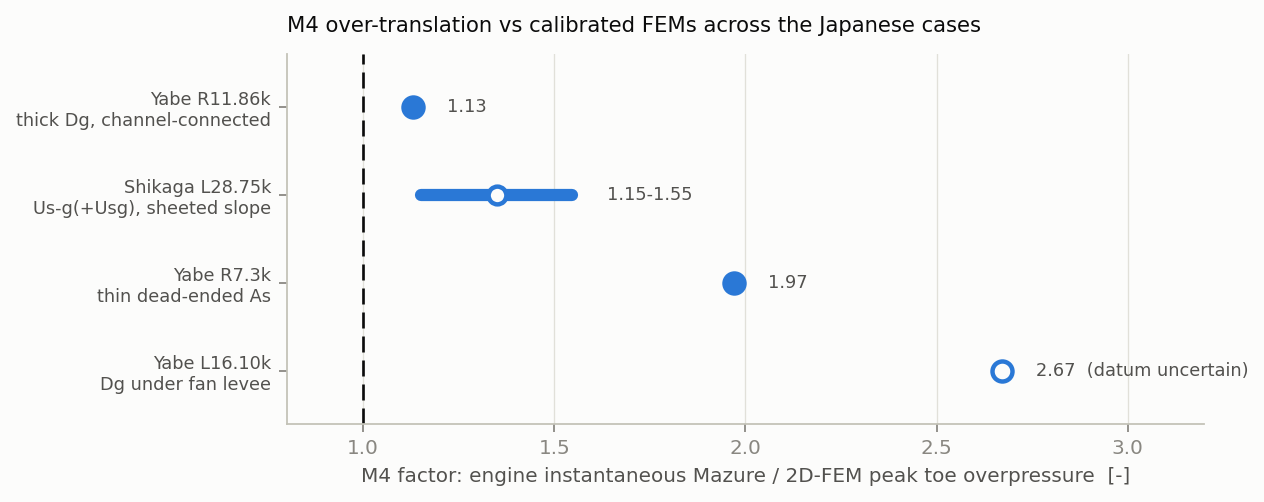
\includegraphics[width=0.85\textwidth]{figures/validation_shikaga_m4_pattern.png}
\caption{Engine instantaneous Mazure translation versus calibrated
two-dimensional FEM peak toe overpressure at the four FEM-anchored Japanese
sites. The pattern tracks aquifer connectedness and storage state; the
shaded band marks the expected position of the Tokachi production sections.}
\label{fig: m4 overtranslation pattern}
\end{figure}

For the Tokachi production runs the judgment is that this bias is not a
blocker, on four grounds. First, all four production sections sit at the
well-matched end of the pattern: confined, perennially channel-connected
coarse aquifers, saturated at base flow, with transmissivities an order of
magnitude above the best-matched Japanese site, and with conditioning
records initialized at the base-flow trough so no fill transient exists to
be mis-modeled; the expected Tokachi factor is approximately
$1.0$--$1.15$. Second, since the raw-head revisions (ADR-0027/0028) the
response factor drives only the uplift and heave gate, never a piping head,
so any residual over-translation opens the erosion window early and is
strictly conservative for the transient failure probability. Third, the
effect is bounded and shoulder-confined: even a hypothetical factor-two
error relocates the mean-value onset head from roughly half the design-level
head to its full value at the governing sections, which shifts the lower
shoulder of the fragility curve while leaving the body, where the gate is
open under either translation for most of the record, essentially unchanged.
Fourth, the bound will be converted into a measured quantity: a sensitivity
member with the response factor halved at KP\,58.8 is registered for the
next production sweep. The residual caveat is inherited by any future
section or replay event featuring dead-ended permeable lenses or entry
through an elevated dry foreland; such cases fall outside the amended
diagnostic's scope and require a transient-fill assessment.

\subsection{The Transient Race Condition Has Field Support}
\label{subsec: The Transient Race Condition Has Field Support}

The scientific core of Phase~1 is the claim that time matters: that failure
is a race between pipe (or cavity) progression and the finite duration of
the load, which the static comparator cannot represent. The Yabe case is the
only one in the set with a breach, and it tests exactly this claim twice.

First, discrimination. Under the same flood, with every site initiating (as
observed: boils appeared at all three), the full engine chain assigns breach
probabilities of $0.061$ at the section that breached, $0$ (in $10^5$
realizations) and $0.005$ at the two that survived. Initiation-level
indicators cannot make this separation: the committee's own $G/W$ minimum at
the breached section ($0.62$) is essentially equal to that at a surviving one
($0.65$). The separation lives in the progression physics, thin fine sand
against thick coarse gravel, and the committee's own explanation of the
survivals is the same rate argument: the surviving foundations' larger
grains and greater thickness made void progression toward the levee slower
\parencite{yabe_levee_committee_2013}. The static branch also ranks the
three sites correctly but leaves an order of magnitude more failure mass at
the undamaged survivor; the transient branch is the sharper discriminator
precisely where sharpness matters.

Second, the timeline. The committee documentation brackets initiation
(FEM uplift onset at 02:00--07:00, the latter independently corroborated by
hinterland wells surging from 07:00) and the breach (13:15--13:30, by CCTV
and firefighters), giving the only field-measured initiation-to-breach
interval in the campaign, approximately $6.3$~h. With the progression clock
forced to the committee initiation anchors, so that the known initiation
conservatism cannot contaminate the test, the Pol rate law under the
\textcite{pol_sie_2024} field prior for $C_e$ brackets this interval across
the committee's own permeability ladder: the probability of a full breach
within the observed interval rises from $0.04$ at the central permeability
(an upper-tail event overall, although the realizations that do breach do so
on the observed clock, with a median time of $6.1$~h against the observed
$6.3$~h) through $0.41$ at an intermediate value to $0.90$ at the coarse,
trench-confirmed permeability of the pathway actually connected to the
river, where the model is typically faster than observed. The single
observed breach therefore sits on the fast side of the
$C_e$ prior. No recalibration is drawn from one event, but the direction is
recorded for Phase~2: survival-driven filtering will pull $C_e$ downward,
and this observation is the counterweight demonstrating that the prior's
width at the fast end carries real mass.

\subsection{The Static Comparator Is Conservative at Every Surviving Site}
\label{subsec: The Static Comparator Is Conservative at Every Surviving
Site}

Across the campaign, wherever the static and transient branches disagree
materially, the observed outcome sided with the transient branch. At
Gounokawa Shimohara the static comparator places up to $25\%$ exceedance
probability (at the base-width seepage length) against three observed
survivals; at Yabe L16.10k it places $13\%$ at a site with no levee
deformation; at Shikaga it places $62$--$99\%$ at a site that survived with
boils only; in each instance the transient branch keeps the survival
probability at $85\%$ or above. At the one breached site both branches place
substantial mass, so the record never contradicts the static branch at a
failure, it only overrules it at survivals. This is the direction Phase~1's
first sub-question hypothesizes, now with field support in the Japanese
setting. The evidential weight must be stated honestly: each survival is a
single Bernoulli observation, so this is a consistent directional pattern
across four sites, not a measured bias factor. The measured bias remains the
Phase~1 fragility-curve comparison itself; the field record's role is to
show the sign is right where it can be checked.

\subsection{Two Structural Findings}
\label{subsec: Two Structural Findings from the Japanese Cases}

\paragraph{No discrete pipe, three investigations out of three.} Every
well-investigated site in the campaign was examined for the pipe the
Sellmeijer--Pol abstraction posits: a trench through the largest Gounokawa
sand volcano found a vein-and-clod complex in the blanket and no pipe at the
erodible interface; the Tokoro test pits found networked sand-filled cracks
and explicitly no water path; the Yabe excavation found the sand layer
intact in section, with the committee mechanism being fines washout growing
cavities beneath the levee. The consistent field object is a distributed
vein, crack, or cavity system, not a discrete horizontal pipe. The working
interpretation adopted here is that the Pol model functions as an effective
rate law for concentrated-seepage damage accumulation, and it performs well
in that role (the Yabe timeline above), but its state variable $l$ should
not be read as the length of a literal conduit. Two practical consequences
are carried through this thesis: trench nulls constrain the model only
weakly, and the structural endpoint $l \geq L/2$ (damage reaching beneath
the crest) is reported alongside the nominal breach endpoint $l \geq L$
wherever field comparisons are made.

\paragraph{Layered foundations force the framework--matrix distinction
everywhere.} The two-population treatment adopted for the Tokachi priors
(ADR-0012), in which the conductivity of the coarse framework and the grain
size of the erodible matrix are treated as properties of different
populations, recurred in every Japanese case as a requirement rather than a
choice. At Gounokawa Shimohara, assigning the gravel's conductivity to the
Sellmeijer and Pol kernels is falsified in both directions at once (it
predicts boiling below a stage the levee had already survived without
ejecta, and near-certain breach against three survivals), while the
erodible sand layer's properties restore consistency; the pressure
translation meanwhile requires the gravel. At Yabe the breach verdict
hinges on pairing the committee's framework conductivity with the
matrix grain size within a single layer. The general statement is that in a
layered foundation the conductivity entering the hydraulic translation
belongs to the transmissive unit, while the conductivity and grain size
entering resistance and erosion belong to the eroding unit. The engine's
single $k_{aq}$ cannot express this split; the validation harnesses realized
it through the public kernels. Whether it becomes an engine capability is
held as a documented candidate decision, to be taken against the OYO logs;
none of the four production sections currently exhibits the
sand-over-gravel stacking that forces it.

\subsection{Transfer to the Tokachi Sections}
\label{subsec: Transfer to the Tokachi Sections}

What transfers. The initiation criterion arrives at Tokachi with its
strongest possible endorsement short of local piezometry: five FEM-anchored
instances, including boiling thresholds in thin covers over coarse
foundations, and a Hokkaido instance (Tokoro) on paleochannel and
confluence deposits that are the closest geological analog to the Tokachi
foundation in the entire set. The Tokoro pattern, boils where the cover is
locally thin, under long-duration stages above the design level, is
precisely the $\gamma'_{bl} D_{bl}$ control the engine encodes. The
hydraulic translation transfers with a characterized, conservative,
bounded error, and the Tokachi sections sit in the regime where that error
is smallest. The progression rate law transfers with one in-domain field
anchor: the Yabe aquifer's matrix grain size ($d_{70} \approx 0.35$~mm) and
seepage length ($\approx 30$~m) are close to the Tokachi matrix values, and
the rate law reproduced the one observed breach clock within its prior.

What does not transfer, or transfers with caveats. The critical heads
computed for the coarse Japanese survivor foundations ($d_{70}$ of
millimeters) lie far outside the \textcite{sellmeijer_2011} calibration
domain; only their direction (coarse means stall) is used, and the same
caveat attaches to the Tokachi bulk-$d_{70}$ co-primary interpretation
wherever it leaves the calibrated range. The timeline validation of $C_e$
rests on a single event conditioned on committee model anchors, and on a
permeability whose in-layer heterogeneity spans the verdict; it supports
the prior's range, not any particular value. The morphology finding implies
that Phase~2 posterior statements about $l$ under the 2016 record inherit
the effective-rate reading, not a literal-conduit one. Finally, the
campaign contains no case combining Tokachi's aquifer thickness with its
flashy multi-peak loading; the compound-event memory model was exercised
(the Yabe record spans two precursor peaks) but its cross-event form was
tested only qualitatively, where the observed re-ejection of Gounokawa
boils at declining heads across three years reflects blanket-pathway
memory, a state the engine deliberately does not carry, and the engine's
prediction of an unchanged virgin threshold is the documented, expected
disagreement.

Taken together, the campaign establishes that the engine's initiation
criterion and progression race condition are sound in the high-gradient
Japanese setting on the evidence available, that its known conservatisms
are localized (head translation) and bounded (gate-only, shoulder-
concentrated), and that the static comparator's conservatism, the premise
of this thesis's central bias question, is visible in the field wherever
the record permits a check.
